\documentclass[sigconf]{acmart}
% defining the \BibTeX command - from Oren Patashnik's original BibTeX documentation.
\def\BibTeX{{\rm B\kern-.05em{\sc i\kern-.025em b}\kern-.08emT\kern-.1667em\lower.7ex\hbox{E}\kern-.125emX}}
% Remove the annoying stuff
\settopmatter{printacmref=false} % Removes citation information below abstract
\renewcommand\footnotetextcopyrightpermission[1]{} % removes footnote with conference information in first column
\pagestyle{plain} % removes running headers



\usepackage{Nikolai}





\begin{document}

%
% The "title" command has an optional parameter, allowing the author to define a "short title" to be used in page headers.
\title{CMIS Hand-in 6: Finite Volume Method}

\author{Nikolai Plambech Nielsen}
\email{lpk331@alumni.ku.dk}
\affiliation{%
  \institution{Niels Bohr Institute, University of Copenhagen}
}


\maketitle

\section{Finite Volume Method}
The finite volume method uses the approximation of piecewise integrals to solve a partial differential equation. One takes the governing equation and integrates it over some finite, fixed volume $ V $. Now one can split the volume into several smaller volumes, called \textit{control volumes}. One can then use numerical approximations to evaluate the integral and obtain a set of linear equations for each control volume. These equations can then be gathered into one matrix and solved for the unknown field.

In this case we are solving a magnetostatics problem. We have a domain $ S $ defined for $ x \in [-3, 3] $ and $ y \in [-1, 1] $, where we have a magnetisation on the unit disc defined as

\begin{equation}\label{key}
	\V{M} = \begin{cases}
	(0, -1)^T, &  x^2+y^2 \leq 1 \\
	(0,0)^T, & \text{otherwise},
	\end{cases}
\end{equation}
with no charges or currents. In this case Maxwells equations read
\begin{equation}\label{key}
	\grad \D \V{B} = 0, \quad \grad \times \V{H} = 0
\end{equation}
The magnetic field $ \V{B} $ is given by
\begin{equation}\label{key}
	\V{B} = \mu_0 ( \V{M} + \V{H})
\end{equation}
and the auxiliary field $ \V{H} $ can be written as the negative gradient of a scalar field, due to the condition of no rotation: $ \V{H} = -\grad \phi $. Putting all this into the equation for the divergence of the magnetic field gives
\begin{equation}\label{key}
	\grad \D \V{B} = \mu_0(\grad \D \V{M} - \grad^2 \phi) = 0
\end{equation}
giving us the governing equation for this system:
\begin{equation}\label{key}
	\grad^2 \phi = \grad \D \V{M}.
\end{equation}
Further, we impose the boundary conditions of
\begin{equation}\label{key}
	\phi(0,1) = 0, \quad \grad\phi\D \V{n} = 0 \quad \forall \V{x} \in \Gamma
\end{equation}
where $ \V{n} $ is the outward unit normal of the domain surface $ S $, and $ \Gamma = \partial S$ is the boundary of the domain.

The approach of the finite volume method is then to integrate the governing equation over the domain and split this integral into control volumes and manipulate the equation a bit:
\begin{align}
	\int_S \grad \D (\grad \phi - \V{M}) \ud S &= \sum_{v \in S} \int_{S_v} \grad \D (\grad \phi - \V{M}) \ud S \\
	&= \sum_{v \in S} \int_{\Gamma_v} (\grad \phi - \V{M}) \D \V{n}\ud \Gamma \\
	&= 0.
\end{align}
Where $ S_v $ denotes a control volume. In the second equality we make use of the Gauss divergence theorem to convert a surface integral into a line integral. Now, the governing equation must hold all over the domain, and as such, so must the integral equation over each control volume. This means that we obtain an equation for each control volume:
\begin{equation}\label{key}
	\int_{\Gamma_v} (\grad \phi - \V{M}) \D \V{n}\ud \Gamma = 0.
\end{equation}
Next we further split the line integral over the control volumes boundary into smaller integrals - one for each edge on the boundary:
\begin{equation}\label{key}
	\int_{\Gamma_v} (\grad \phi - \V{M}) \D \V{n}\ud \Gamma = \sum_{e \in \Gamma_v} \int_{\Gamma_e} (\grad \phi - \V{M}) \D \V{n}\ud \Gamma = 0
\end{equation}
We now introduce the integral average of a quantity:
\begin{equation}\label{key}
	\overline{f(x)} = \frac{1}{b-a} \int_{a}^{b} f(x) \ud x 
\end{equation} 
and rewrite the integrals as
\begin{equation}\label{key}
	\sum_{e \in \Gamma_v} \int_{\Gamma_e} (\grad \phi - \V{M}) \D \V{n}\ud \Gamma = \sum_{e\in \Gamma_v} (\overline{\grad\phi} - \overline{\V{M}} )\ell_e = 0
\end{equation}
where $ \ell_e $ is the length of the $ e $'th edge. Assuming each edge is short, we approximate the integral using the midpoint rule:
\begin{equation}\label{key}
	\int_{a}^{b} f(x) \ud x \approx (b-a) f\pp{\frac{b-a}{2}}
\end{equation}
With this approximation, the integral average becomes just the value of the integrand at the midpoint of the edge. This makes sense, since we are essentially saying that the integrand is constant over the integration range, and so the average is precisely this constant. All we need now, is a way to calculate the midpoint value, and then we are set to solve the problem!

\subsection{Control volumes}
\begin{figure}
	\centering
	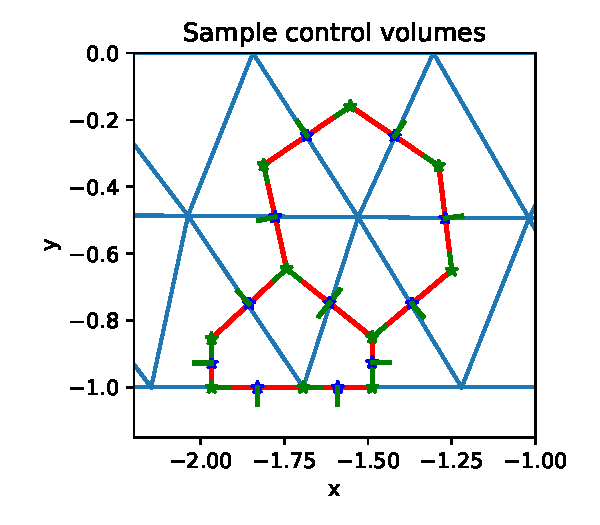
\includegraphics[width=\linewidth]{control_volumes.pdf}
	\caption{Sample vertex centred dual control volumes for the computational mesh. Triangle mesh is blue, control volumes are red. green points denote vertices of the control volumes. The centre of the upper control volume is an inner node of the triangle mesh, and the control volume is therefore a hexagon. The centre of the lower control volume is a boundary node of the triangle mesh, and therefore has boundary edges.}
	\label{fig:control_volumes}
\end{figure}
Now, we have used the words control volume and made reference to its edges along the boundary. In general a control volume is any fixed, finite volume in the domain. We of course need the union of all control volumes to be exactly the whole domain, otherwise the solution obtained will not be a solution to the problem posed.

One could use a mesh of triangles, quadrilaterals, or any other shape, for that matter. The choice depends on where one stores the values of the unknowns as well as ease of computability. In our case we use a triangular mesh, where we store the values of $ \phi $ on the vertices, and use a vertex centred dual control volume. 

This means that for each vertex in our mesh, we compute the incenters of all triangles the vertex is a part of, and join these together. If the vertex is on the boundary of the domain, we join the incenter of the two boundary triangles to the nearest point on the boundary. See figure \ref{fig:control_volumes} for an example.


\subsection{Approximations}
\begin{figure}
	\centering
	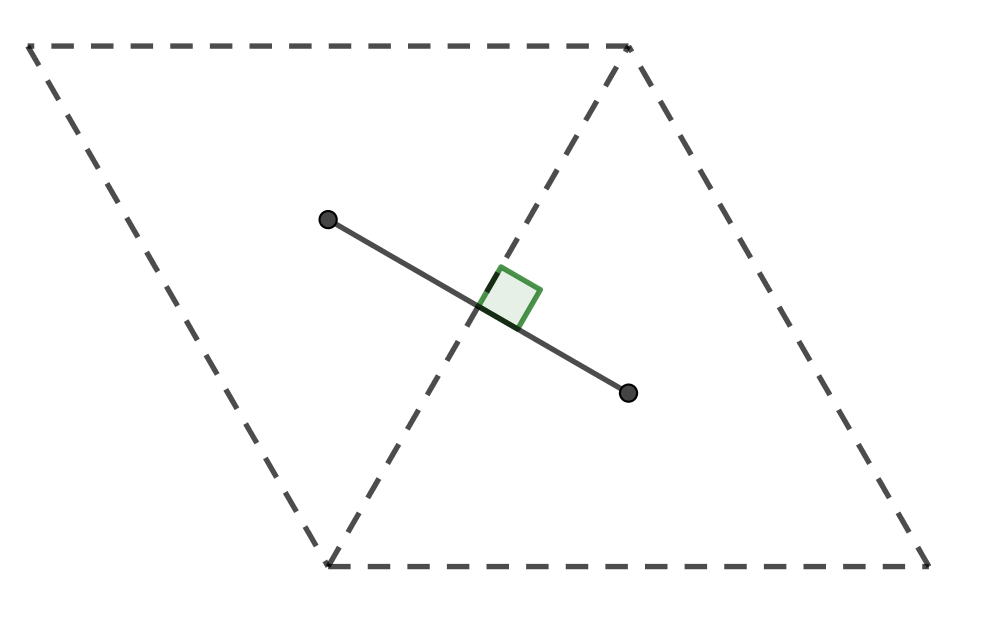
\includegraphics[width=0.7\linewidth]{triangles.png}
	\caption{Incentres and surface normals for equilateral triangles. The line between incentres is perpendicular to the line joining the two vertices shared by the two triangles.}
	\label{fig:triangles}
\end{figure}
This choice of control volumes gives us an easy way of calculating the directional derivative $ \grad\phi \D \V{n} $, under the assumption that the triangles are close to being equilateral. If the triangles are equilateral, then the line joining the incenters of two adjacent triangles will also be the perpendicular bisector between the two vertices shared by the triangles (see figure \ref{fig:triangles}). This then means that the directional derivative from the $ i $'th vertex to the $ j $'th vertex can be approximated easily using a finite difference:
\begin{equation}\label{key}
	\grad \phi \D \V{n} \approx \frac{\phi_j - \phi_i}{|\V{x}_i-\V{x}_j|}
\end{equation}
Of course as the triangles become ``less'' equilateral, this approximation will be more erroneous. This is evident in figure \ref{fig:control_volumes} where the outward surface normals between the two control volume do not line up with the straight line segment between two control volume centres.

Further, when considering edges which end on the boundary of the domain we have no easy way of calculating the directional derivative at the midpoint of the edge. We therefore use the zeroth order approximation that the value at the midpoint is the same as that at the end point - precisely the same equation as above.

If the edge of the control volume is along the boundary of the domain, we need to apply the boundary condition $ \grad \phi \D \V{n} = 0$. We can use the value of $ \phi $ at the end point with a incenter perpendicular to the boundary (call it $ \phi_e $), along with the value of $ \phi $ at the incenter to estimate the directional derivative (call it $ \phi_c $).

We approximate the two values as
\begin{equation}\label{key}
	\phi_c = \frac{1}{3} (\phi_i + \phi_j + \phi_k) \quad \phi_e = \frac{\phi_j-\phi_i}{x_j-x_i} (x_e-x_i) + \phi_i 
\end{equation}
ie the value of the incenter is the mean of the vertex values, and the value at the edge is linearly interpolated between the vertices on the edge (see figure \textbf{REF}). The directional derivative is then approximated by
\begin{equation}\label{key}
	\grad\phi \D \V{N} \approx \frac{\phi_e - \phi_c}{|\V{x}_e - \V{x}_c|} = \frac{\phi_i \pp{\frac{4}{3} + \frac{x_e-x_i}{x_j-x_i}} + \phi_j \pp{\frac{1}{3} + \frac{x_e-x_i}{x_j-x_i}} + \frac{\phi_k}{3}}{|\V{x}_c - \V{x}_e|}
\end{equation}
For the source term we just put a 0.


Putting all these considerations together we get the equation for the $ i $'th control volume (with $ i $ not being a boundary vertex):
\begin{equation}\label{key}
	\sum_{e \in \Gamma_v} \frac{\phi_{j(e)}-\phi_i}{|\V{x}_i - \V{x}_{j(e)}|} \ell_e = \sum_{e\in \Gamma_v} \V{M}_e \D \V{n}_e.
\end{equation}
where $ j(e) $ is the neighbouring vertex corresponding to the edge segment $ e $, $ \V{M}_e $ is the value of $ \V{M} $ at the midpoint of the edge and $ \V{n}_e $ is the outward surface normal of the $ e $'th edge segment.

Now, $ \V{M} $ has a discontinuity around the unit disc. If an edge intersects this (ie, one end is inside, whilst the other is outside), then using the midpoint value of $ \V{M} $ no longer gives an accurate integral. Instead we split the integral into two:
\begin{equation}\label{key}
	\int_{\V{x}_i}^{\V{x}_j} \V{M}\D \V{n} \ud \Gamma = \int_{\V{x}_i}^{\V{p}} \V{M}\D \V{n} \ud \Gamma + \int_{\V{p}}^{\V{x}_j}\V{M}\D \V{n} \ud \Gamma
\end{equation}
where one of these is 0. The intersection $ \V{p} $ is calculated with
\begin{equation}\label{key}
	p_x = \frac{D d_y \pm \sign( d_y) d_x \sqrt{r^2 d_r^2 - D^2}}{d_r^2}, \quad p_y = \frac{-D d_x \pm |d_y| \sqrt{r^2 d_r^2 - D^2}}{d_r^2}
\end{equation}
with $ d_y = y_i-y_j, d_x = x_i - x_j, d_r = \sqrt{d_x^2 + d_y^2} = \ell_e , D = x_i y_j-x_jy_i$, as per \href{http://mathworld.wolfram.com/Circle-LineIntersection.html}{Wolfram Alpha}. We only need the one intersection, defined by the equation
\begin{equation}\label{key}
	p_x = x_i + s(x_j - x_i) \quad s = \frac{p_x-x_i}{x_j-x_i}
\end{equation}
if $ 0\leq s \leq 1 $, then we have the right intersection, as $ x_i \leq p_x \leq x_j $, which implies the same for $ p_y $.

The $ \V{M} $-integral for that side is then
\begin{equation}\label{key}
	\int_{\V{p}}^{\V{x}_j}\V{M}\D \V{n} \ud \Gamma = (\V{M}_{\text{in}} \D \V{n}) |\V{p}-\V{x}_j|
\end{equation}
where we assume $ \V{x}_j $ is inside the unit disc and $ \V{x}_i $ is outside. The left hand ($ \phi $) integral remains the same, of course, as $ \phi $ is assumed continuous.

Another way to handle this would be to alter the mesh, such that no control volume edges cross the unit disc. However, when using the vertex centered dual control volume, constructing the mesh such that this happens is much more of a challenge than simply putting in an if statement in the code and call it a day, even if the equations for the circle intersection are slightly cumbersome.


\subsection{Matrix assembly}
With the theory in place, it is time to assemble the system of equations. We have $ N $ vertices in the system and therefore $ N $ control volumes, each with one linear equation relating the $ N $'th vertex to its neighbours. We therefore start with a $ N\times N $ matrix, $ A $, of zeros. In the $ i $'th row we add the value $ \ell_e/|\V{x}_i-\V{x}_{j(e)}| $ in all the columns corresponding to neighbours, and minus the sum of all the others values in the $ i $'th diagonal element.

For the source term $ \V{b} $ we start with a $ N $-vector of zeros as above, and add the sum of $ \V{M} $-integrals above, taking care to split any integrals crossing the discontinuity of $ \V{M} $.

With the matrix and source term we can then easily compute the solution $ \phi $ to the problem using a direct solver (assuming, of course, we have a non-singular matrix, which the boundary conditions should take care of).

This is all highly reminiscent of the matrix assembly for both FEM and FDM.

\section{Experiments}
\begin{figure}
	\centering
	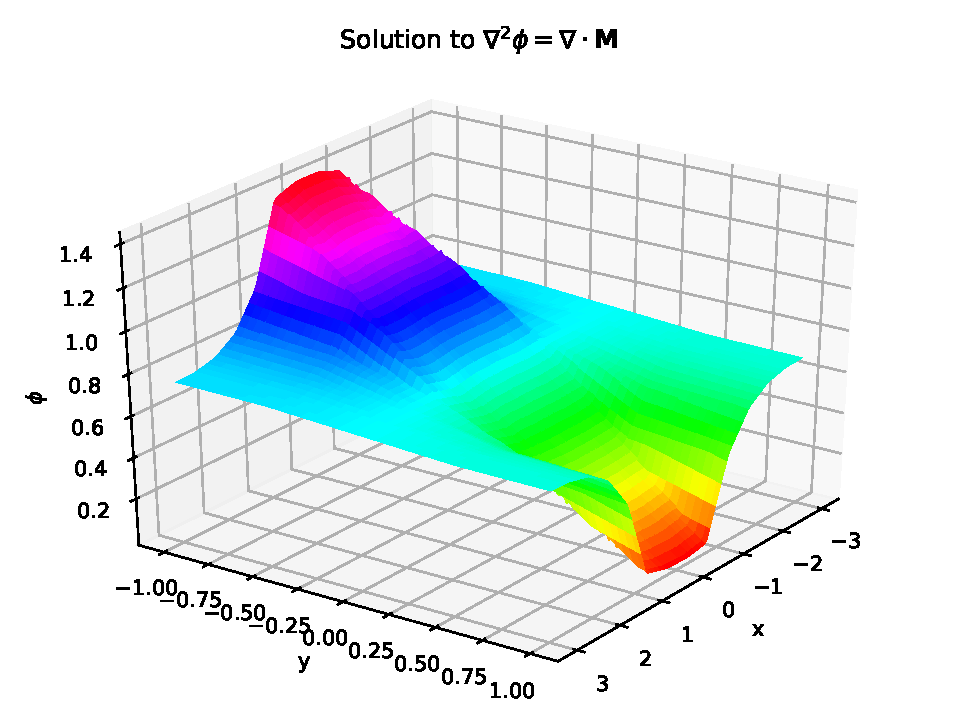
\includegraphics[width=\linewidth]{ex_simple.pdf}
	\caption{Solution to the magnetostatics problem with a unit disc of magnetised material. Indeed we see a scalar potential in the vicinity of the unit disc.}
	\label{fig:ex_simple}
\end{figure}
\begin{figure}
	\centering
	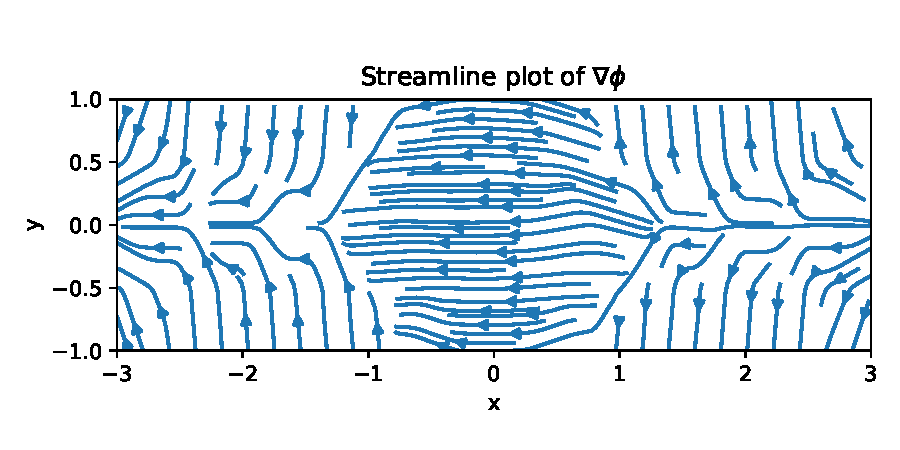
\includegraphics[width=\linewidth]{ex_streams.pdf}
	\caption{Streamline plot of the gradient of $ \phi $. Note the slightly hexagonal look of the unit disc.}
	\label{fig:ex_streams}
\end{figure}
First of all, let us plot the solution to the problem obtained using the method outlined above, on the sample mesh for this week. The result is seen in figures \ref{fig:ex_simple} and \ref{fig:ex_streams}. As we see, we have a a region around the unit disk with a non-zero scalar potential, while it is approximately zero ``far'' away from the disk. This precisely the expected behaviour from magnetostatics and electrostatics. Further more, on the streamplot of the gradient of $ \phi $ (the electrical field) we see that the gradient is perpendicular to the magnetisation, as one usually expects in the case for induced fields. Overall, the solution makes physical sense.

A thing to note, which is especially visible in the streamline plot: the unit ``disc'', which should be visible looks more like a unit ``hexagon'', which is most likely an artefact of the somewhat low resolution mesh used. Upping the resolution should remedy this.

Since the governing equation has reflective or parity symmetry we should expect the solution to be the same for a flipped $ x $-coordinate: $ \phi(x, y) = \phi(-x, y) $. Similarly, if we flip the sign of $ \V{M} $ and perform a parity transform in $ y $, we should also expect the same solution (essentially charge conjugation / parity (CP) symmetry), so long as we also change the boundary condition of $ \phi(0,1) =0 $ to $ \phi(0,-1)=0 $, as this fixes the offset between the scalar potentials (and as we know, we can always add and subtract constants to our potentials - it is always the gradient that matters!).
\begin{figure}
	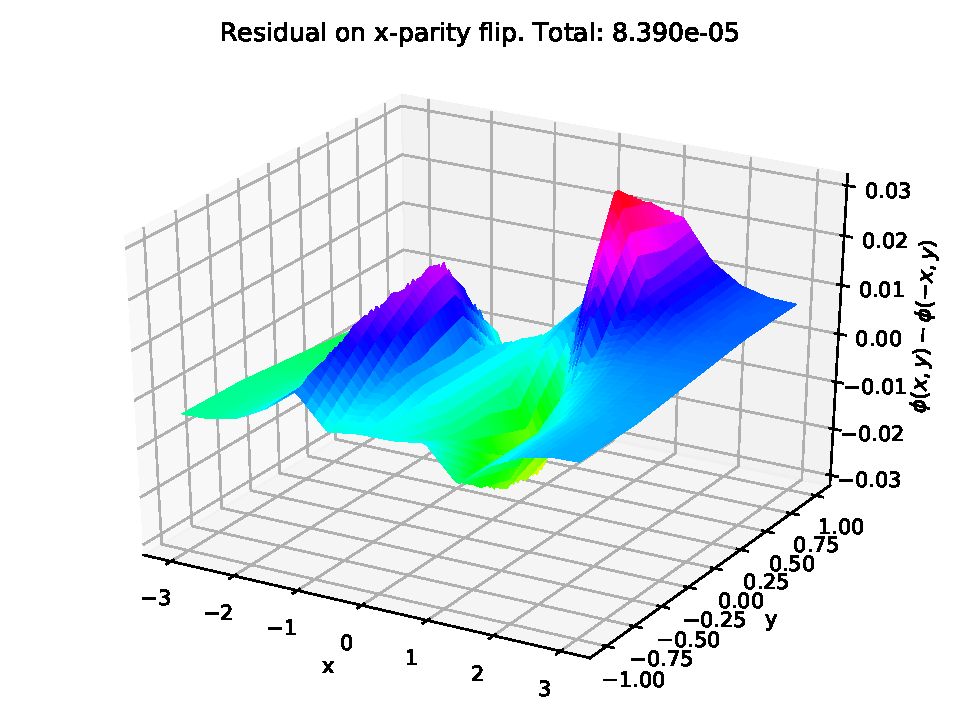
\includegraphics[width=\linewidth]{ex_res_x.pdf}
	\caption{Residual upon a parity transformation in $ x $.}
	\label{fig:xres}
\end{figure}
To easily calculate the residual $ \phi(x)-\phi(-x) $ we first interpolate $ \phi $ to a grid, making sure that when we reflect $ x $ each point lands on top of its ``parity partner'', then we subtract $ \phi $ from $ \phi $, where we just reverse the direction of the columns (remember, that in Python, by default $ x $ is the second index). We then square each difference, sum up and divide by the total number of points to get the final residual. The result is seen in figure \textbf{ref}. If we sum $ \phi $ over the domain and divide by the number of points we get 0.7136, which means the residual is around 4 orders of magnitude smaller than the ``integral''. There is also a small yet noticeable asymmetry in the $ x $-direction of the residual. With a residual of this size we still conclude, however, that there is at least approximate parity symmetry in $ x $ for the solution.

\begin{figure}
	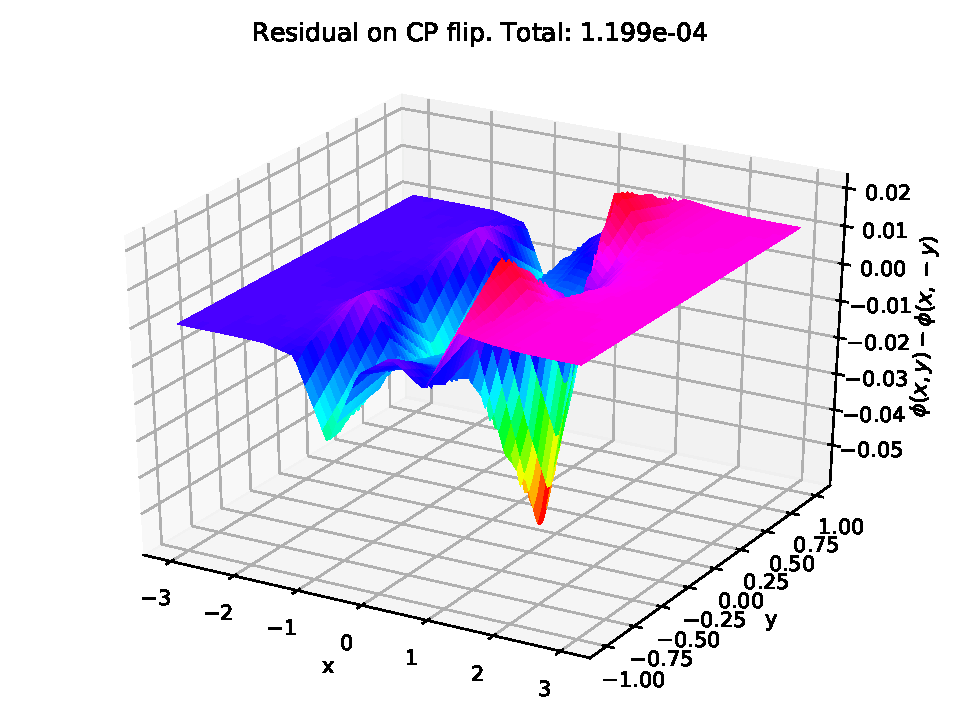
\includegraphics[width=\linewidth]{ex_res_y.pdf}
	\caption{Residual upon a CP-like transformation. Note the distinct asymmetry in the residual.}
	\label{fig:yres}
\end{figure}
For the $ y $-residual we flip the sign on $ \V{M} $ when creating the source term vector, and change the boundary condition as written above. Then we calculate the new solution and compare the first to the second, with the first argument reversed, corresponding to $ \phi(x,y)-\phi(x,-y) $. The result is seen in figure \textbf{ref}. Again, there is a small residual, though larger than the one for $ x $-parity. It is still roughly 3 orders of magnitude smaller than the ``integral'', but we also see a distinct asymmetry in the $ x $-direction like for the $ x $-parity, yet larger. The result is not quite as clear cut as for the $ x $-parity, but it is still definitely in the ``right'' direction. Maybe a higher resolution grid would produce a better result.



\end{document}

